\documentclass[]{beamer}
\usepackage[T1]{fontenc}
\usepackage[utf8]{inputenc}
\usepackage{lmodern}
\usepackage[italian]{babel}

\title{La corrente elettrica continua}
\author{\texorpdfstring{Mattia Cozzi\newline\href{mailto:cozzimattia@gmail.com}{\texttt{cozzimattia@gmail.com}}}{Mattia Cozzi}}
\date{a.s.~2023/2024}

%\documentclass[handout]{beamer}     %usare questa classe per generare l'handout
%\usepackage{pgfpages}   %per mostrare più quadri nella stessa pagina
%\pgfpagesuselayout{4 on 1}[a4paper,border shrink=5mm,landscape]
\usetheme{Singapore}
%\useoutertheme[left]{sidebar} %elementi intorno alle diapositive
\setbeamercovered{dynamic} %modifica l'aspetto del testo grigetto delle diapositive future. Argomenti: invisible/transparent/dynamic
\usecolortheme{orchid}
%COLORE PRINCIPALE
% \definecolor{marroncino}{RGB}{156, 26, 0} % UBC Blue (primary)
% \setbeamercolor{structure}{fg=marroncino} % itemize, enumerate, etc

\theoremstyle{plain}
\newtheorem{teorema}{Teorema}

\usepackage{tikz}
\usepackage{circuitikz}

\usepackage{pgf,pgfplots,graphicx}
\usetikzlibrary{angles,quotes,arrows,shapes,decorations.markings}
\pgfplotsset{compat=1.15}
\usepgfplotslibrary{units,fillbetween} % to add units easily to axis

\newcommand{\fem}{f_{em}}
\usepackage{booktabs}
\begin{document}

\begin{frame}
  \titlepage
\end{frame}





\begin{frame}
\frametitle{Contenuti}
\tableofcontents
\end{frame}


\section{Corrente}





\begin{frame}
\frametitle{La corrente elettrica}
\begin{block}{Corrente elettrica}
Una corrente elettrica è un moto \emph{ordinato} di cariche elettriche.
\end{block}\pause
\begin{block}{Intensità di corrente elettrica}
L'intensità di corrente si misura in \emph{ampere} (simbolo $A$) e vale:
\begin{center}
\colorbox{blue!30}{$ i = \dfrac{\Delta q}{\Delta t} $}
\end{center}
\end{block}\pause
\begin{block}{Corrente elettrica continua}
Una corrente elettrica è continua se la sua intensità non cambia nel tempo.
\end{block}\pause
L'intensità di corrente si misura con un \emph{amperometro}.
\end{frame}


\begin{frame}
\frametitle{Il verso della corrente}
\begin{figure}
  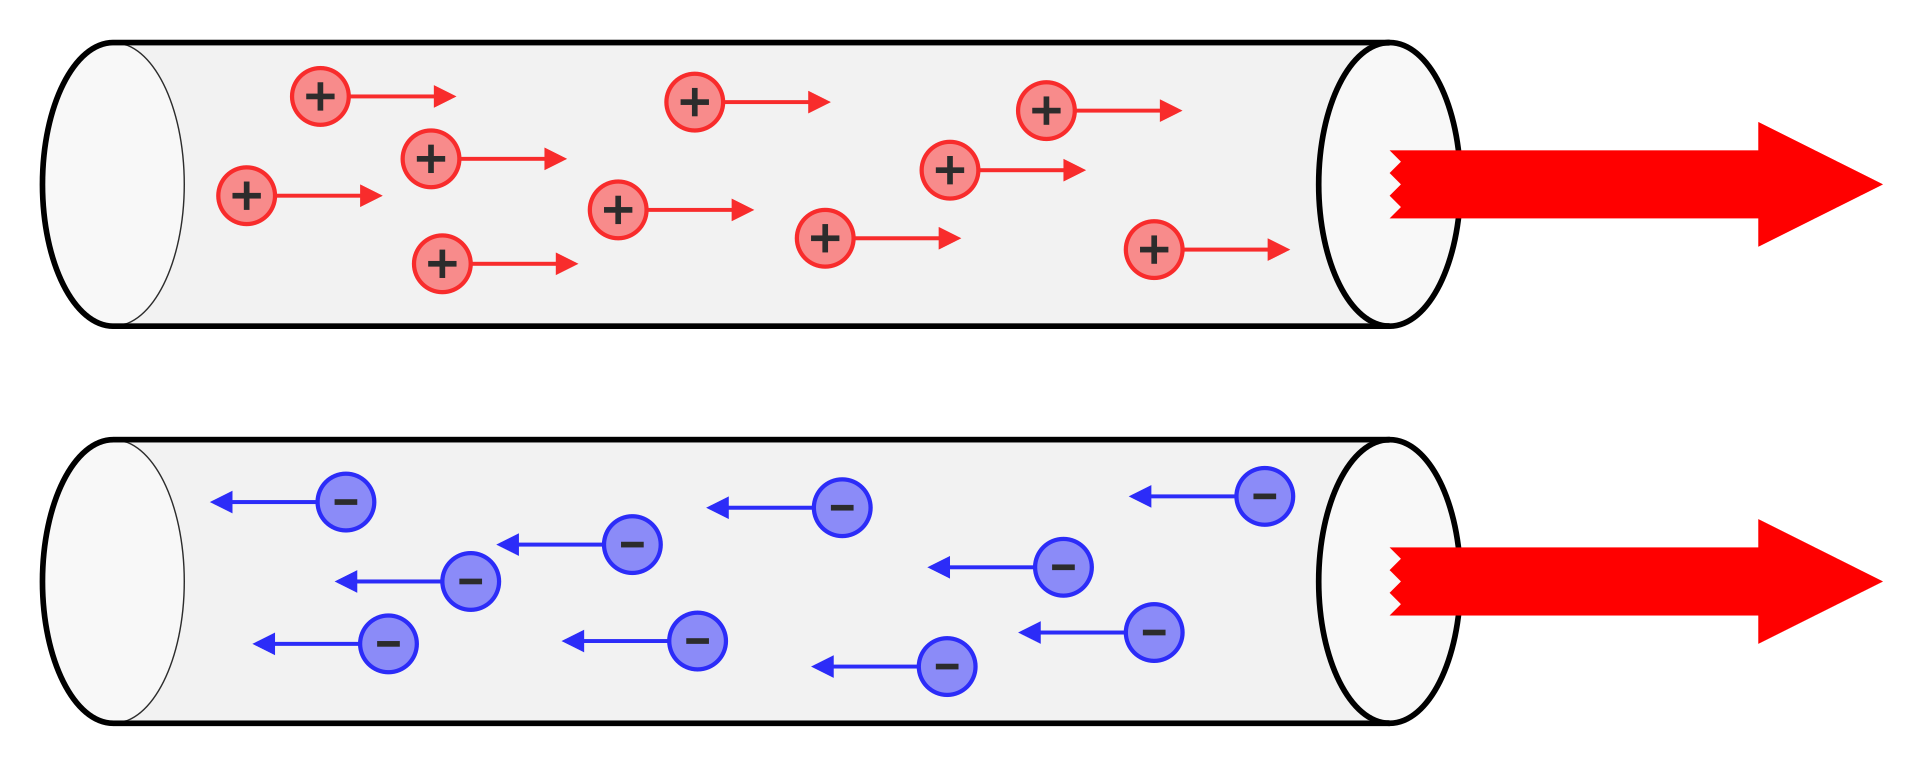
\includegraphics[width=.7\columnwidth]{img/corrente.png}
\end{figure}
\begin{alertblock}{Attenzione!}
Il verso della corrente è definito come quello in cui si muovono (o si muoverebbero) le cariche positive.{\pause} Pertanto, se il conduttore è metallico, il verso effettivo del moto degli elettroni è \alert{opposto} a quello della corrente.
\end{alertblock}
\end{frame}



\begin{frame}
\frametitle{Esercizio}
\begin{exampleblock}{Carica che attraversa un filo}
  \small{
  In un filo elettrico circola una corrente di intensità $ 4,0 \times 10^{-2} \, A $ per $ 5,0 \, s $.

  Calcola la carica totale che attraversa una sezione del filo in quell'intervallo di tempo.\hspace*{\fill}[$ 0,20 \, C $]
  
  A quanti elettroni corrisponde tale carica?\hspace*{\fill}[$ 1,3 \times 10^{18} $]}
\end{exampleblock}
\end{frame}



\section{Circuiti}



\begin{frame}
\frametitle{Generatori di tensione}
\begin{block}{Generatore di tensione continua}
È un dispositivo capace di mantenere ai suoi capi una differenza di potenziale o tensione, $ \Delta V $, per un tempo idealmente indeterminato.
\end{block}\pause
Esempi di generatori di tensione sono le pile per i telecomandi ($ \Delta V = 1,5 \, V $) o le batterie per automobili ($ \Delta V = 12 \, V $).
\begin{columns}
\begin{column}{0.2\textwidth}
\visible<2>{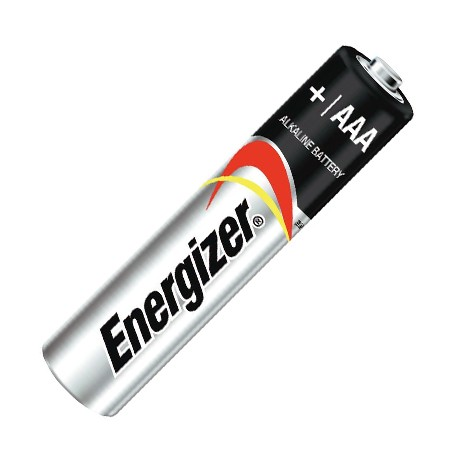
\includegraphics[width=\columnwidth]{img/1,5V.jpg}}
\end{column}
\begin{column}{0.3\textwidth}
\visible<2>{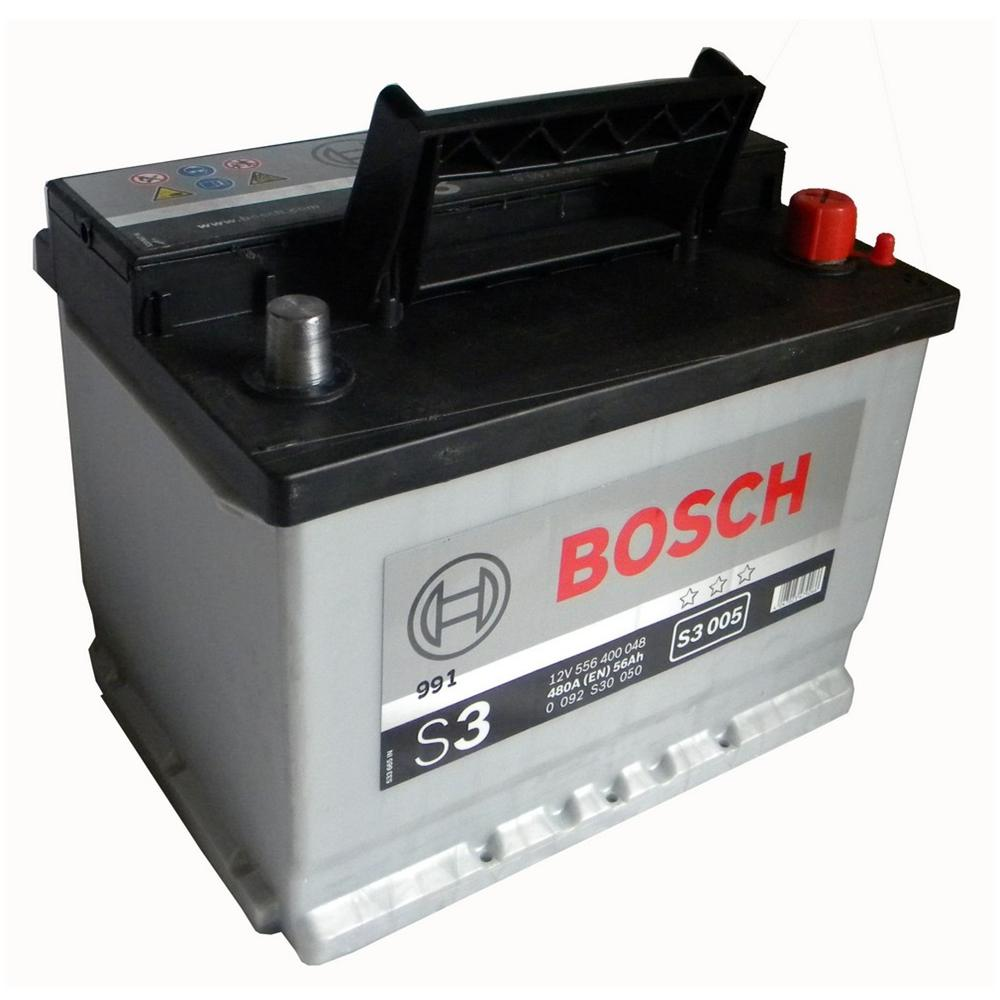
\includegraphics[width=\columnwidth]{img/12V.jpg}}
\end{column}
\begin{column}{0.3\textwidth}
\begin{figure}\centering
\ctikzset{bipoles/length=1.5cm}
\begin{circuitikz}[scale=0.5]
\draw (0,0) to[battery, a=$\Delta V$, *-*] (4,0);
\draw (0,4) to[battery1, a=$\Delta V$, *-*] (4,4);
\end{circuitikz}
\end{figure}
\end{column}
\end{columns}
\end{frame}




\begin{frame}
\frametitle{Elementi di un circuito}
\begin{block}{Circuito elettrico}
Insieme di conduttori connessi in modo continuo e collegati ad un generatore.\pause\\~\\Può essere \emph{chiuso} (passa corrente) o \emph{aperto} (non passa corrente).
\end{block}\pause
Alcuni elementi di un circuito:
\begin{figure}\centering
\ctikzset{bipoles/length=1.0cm}
\begin{circuitikz}[scale=0.4] 
\draw (0,0) to[battery1, l=generatore, *-*] (4,0);
\draw (6,0) to[lamp, l=lampadina, *-*] (10,0);
\draw (12,0) to[push button, l=bottone, *-*] (16,0);
\draw (18,0) to[R, l=resistore, *-*] (22,0);
\draw (0,-5) to[nos, l=interr aperto, *-*] (4,-5);
\draw (6,-5) to[capacitor, l=condensatore, *-*] (10,-5);
\draw (12,-5) to[ammeter, l=amperometro, *-*] (16,-5);
\draw (18,-5) to[voltmeter, l=voltimetro, *-*] (22,-5);
\end{circuitikz}
\end{figure}
\end{frame}



\begin{frame}
\frametitle{Circuito elettrico elementare}

\begin{figure}\centering
\ctikzset{bipoles/length=1.2cm}
\begin{circuitikz}[scale=0.7]
\draw (0,0) to[battery1, l=$\Delta V$](6,0);
\draw (0,0) to[short, f_=$i$] (0,4);
\draw (0,4) to[R, l=R] (6,4);
\draw (6,4) to[short, f_=$i$] (6,0);
\end{circuitikz}
\end{figure}\pause
\begin{block}{Risoluzione di un circuito}
Risolvere un circuito significa individuare il valore e il verso di tutte le correnti presenti e, di conseguenza, anche il valore delle tensioni ai capi di tutti i resistori.
\end{block}
\end{frame}



\section{Resistenza}

\begin{frame}
  \frametitle{La prima legge di Ohm}
  \begin{block}{Prima legge di Ohm}
Nei conduttori ohmici l'intensità di corrente è direttamente proporzionale alla differenza di potenziale applicata ai loro capi.
\begin{center}
\colorbox{blue!30}{$ i = \dfrac{\Delta V}{R} $}
\end{center}\pause
In un grafico $ \Delta V $/$ i $, la quantità $ \dfrac{1}{R} $ è il coefficiente angolare della retta.
\end{block}\pause
  \begin{alertblock}{Resistenza}
La prima legge di Ohm introduce (definisce) una nuova quantità: la resistenza, misurata in \emph{ohm} ($\Omega$).
\end{alertblock}
  
\end{frame}



\begin{frame}
\frametitle{I resistori}
  \begin{block}{Resistore}
Un resistore è un componente elettrico che segue la prima legge di Ohm.
\end{block}
\begin{columns}
\begin{column}{0.3\textwidth}
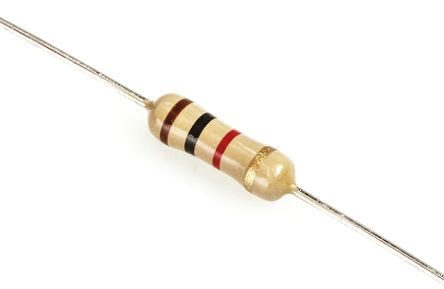
\includegraphics[width=\columnwidth]{img/resistenza1.jpg}
\end{column}
\begin{column}{0.3\textwidth}
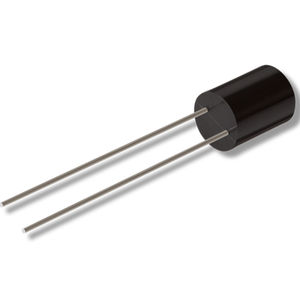
\includegraphics[width=\columnwidth]{img/resistenza2.jpg}
\end{column}
\begin{column}{0.3\textwidth}
\begin{figure}\centering
\ctikzset{bipoles/length=1.5cm}
\begin{circuitikz}[scale=0.5]
\draw (0,0) to[R, *-*] (4,0);
\end{circuitikz}
\end{figure}
\end{column}
\end{columns}
\end{frame}

\begin{frame}
  \frametitle{Esempio 1}

\begin{figure}\centering
\ctikzset{bipoles/length=1.2cm}
\begin{circuitikz}[scale=0.7]
\draw (0,0) to[battery1, l=$\Delta V$, a=?](6,0);
\draw (0,0) to[short, f_=$i$, l=$ 3 \, A $] (0,4);
\draw (0,4) to[R, l=R, a=$ 4 \, \Omega $] (6,4);
\draw (6,4) to[short, f_=$i$, l=$ 3 \, A $] (6,0);
\end{circuitikz}
\end{figure}
\end{frame}


\begin{frame}
\frametitle{Esercizio}
\begin{exampleblock}{Prima legge di Ohm}
  \small{
  Un alimentatore mantiene una differenza di potenziale costante ai propri morsetti. Quando lo si collega ad un resistore da $ 150 \, \Omega $, esso produce una corrente di $ 80 \, mA $. In un secondo momento viene collegato ad un resistore da $ 560 \, \Omega $.

  Calcola la corrente che attraversa il secondo resistore.\hspace*{\fill}[$ 21 \, mA $]}
\end{exampleblock}
\end{frame}

\section{Collegamento}


\begin{frame}
\frametitle{Modalità di collegamento}

\begin{figure}\centering
\ctikzset{bipoles/length=0.6cm}
\begin{circuitikz}[scale=0.5]
\draw (0,0) to[battery1, l=$\Delta V$](6,0);\pause
\draw (0,0) to[lamp, f_=$i$] (0,4);\pause
\draw (0,4) to[lamp, f_=$i$] (6,4);\pause
\draw (6,4) to[lamp, f_=$i$] (6,0);
\end{circuitikz}\pause
\end{figure}

\begin{block}{Collegamento in serie}
Più conduttori sono collegati in serie se sono posti in successione tra loro.\\~\\\pause

Essi sono \alert{attraversati dalla stessa corrente elettrica}.
\end{block}
\end{frame}


\begin{frame}
\frametitle{Modalità di collegamento}

\begin{figure}\centering
\ctikzset{bipoles/length=0.5cm}
\begin{circuitikz}[scale=0.5]
\draw (0,0) to[battery1, a=$\Delta V$, f<=$i$](6,0);
\draw (0,0) to[short] (0,4);
\draw (0,4) to[short, f_=$i$] (2,4);\pause
\draw (2,2.5) to[short] (2,5.5);
\draw (2,5.5) to[lamp, i_=$i_1$] (4,5.5);
\draw (4,5.5) to[short] (4,4);
\draw (2,2.5) to[lamp, i_=$i_3$] (4,2.5);
\draw (4,2.5) to[short] (4,4);
\draw (2,4) to[lamp, i_=$i_2$, o-o] (4,4);\pause
\draw (4,4) to[short] (6,4);
\draw (6,4) to[short, f_=$i$] (6,0);
\end{circuitikz}\pause
\end{figure}

\begin{block}{Collegamento in parallelo}
Più conduttori sono collegati in parallelo se hanno le estremità connesse tra loro.\\~\\\pause
Essi sono \alert{sottoposti alla stessa differenza di potenziale}.
\end{block}
\end{frame}





\begin{frame}
  \frametitle{Collegamento di resistori}
  \begin{block}{Resistenza equivalente}
Si chiama resistenza equivalente $ R_{eq} $ della rete di resistori quella di un singolo resistore che, sottoposto alla stessa differenza di potenziale $ \Delta V $ a cui è soggetta l’intera rete, assorbe dal generatore la stessa corrente elettrica.
\end{block}
\end{frame}



\begin{frame}
\frametitle{Collegamento in serie}

\begin{figure}\centering
\ctikzset{bipoles/length=1.0cm}
\begin{circuitikz}[scale=0.7]
\draw (0,0) to[battery1, l=$\Delta V$](6,0);
\draw (0,0) to[R=$R_1$, f_=$i$] (0,4);
\draw (0,4) to[R=$R_2$, f_=$i$] (6,4);
\draw (6,4) to[R=$R_3$, f_=$i$] (6,0);
\end{circuitikz}
\end{figure}
\begin{center}
\colorbox{blue!30}{$ R_{eq} = R_1 + R_2 + R_3 + ... $}
\end{center}
\end{frame}


\begin{frame}
\frametitle{Collegamento in parallelo}

\begin{figure}\centering
\ctikzset{bipoles/length=0.6cm}
\begin{circuitikz}[scale=0.7]
\draw (0,0) to[battery1, a=$\Delta V$, f<=$i$](6,0);
\draw (0,0) to[short] (0,4);
\draw (0,4) to[short, f_=$i$] (2,4);
\draw (2,2.5) to[short] (2,5.5);
\draw (2,5.5) to[R=$R_1$, i_=$i_1$] (4,5.5);
\draw (4,5.5) to[short] (4,4);
\draw (2,2.5) to[R=$R_3$, i_=$i_3$] (4,2.5);
\draw (4,2.5) to[short] (4,4);
\draw (4,4) to[short] (6,4);
\draw (2,4) to[R=$R_2$, i_=$i_2$, o-o] (4,4);
\draw (6,4) to[short, f_=$i$] (6,0);
\end{circuitikz}
\end{figure}
\begin{center}
\colorbox{blue!30}{$ \frac{1}{R_{eq}} = \frac{1}{R_1} + \frac{1}{R_2} + \frac{1}{R_3} + ... $}
\end{center}
\end{frame}

\begin{frame}
  \frametitle{Esempio 2}
\begin{columns}
\begin{column}{0.4\textwidth}
\visible<1->{
\vspace*{-1 cm}
\begin{figure}\centering
\ctikzset{bipoles/length=1.0cm}
\begin{circuitikz}[scale=0.7]
\draw (0,0) to[battery1, l=$\Delta V$](6,0);
\draw (0,0) to[R, a=$ 3\, \Omega $] (0,4);
\draw (0,4) to[R, a=$ 4\, \Omega $] (6,4);
\draw (6,4) to[R, a=$ 6\, \Omega $] (6,0);
\end{circuitikz}
\end{figure}
\[ R_{eq} = 3 \, \Omega + 4 \, \Omega + 6 \, \Omega = 13 \, \Omega  \]
}

\end{column}
\begin{column}{0.5\textwidth}

\visible<2->{

\begin{figure}\centering
\ctikzset{bipoles/length=.7cm}
\begin{circuitikz}[scale=0.7]
\draw (0,0) to[battery1, l=$\Delta V$](6,0);
\draw (0,0) to[short] (0,4);
\draw (0,4) to[short] (2,4);
\draw (2,2.5) to[short] (2,5.5);
\draw (2,5.5) to[R, a=$ 3\, \Omega $] (4,5.5);
\draw (4,5.5) to[short] (4,4);
\draw (2,2.5) to[R, a=$ 6\, \Omega $] (4,2.5);
\draw (4,2.5) to[short] (4,4);
\draw (4,4) to[short] (6,4);
\draw (2,4) to[R, o-o, a=$ 4\, \Omega $] (4,4);
\draw (6,4) to[short] (6,0);
\end{circuitikz}
\end{figure}
$ \dfrac{1}{R_{eq}} = \dfrac{1}{3\, \Omega} + \dfrac{1}{4\, \Omega} + \dfrac{1}{6\, \Omega} = \dfrac{9}{12\, \Omega} $}

~

\visible<3>{\[ R_{eq} = \dfrac{12}{9} \, \Omega = 1,33 \, \Omega \]
}
\end{column}
\end{columns} 
\end{frame}



\begin{frame}
\frametitle{Esercizio}
\begin{exampleblock}{Resistori in serie}
  \small{
  In un circuito sono collegati in serie un generatore di tensione da $ 18,0 \, V $ e dieci resistori uguali. Viene misurata l'intensità di corrente, che risulta di $ 6,0 \, mA $.

  Calcola il valore della resistenza di ciascun resistore.\hspace*{\fill}[$ 3,0 \times 10^{2} \, \Omega $]}
\end{exampleblock}
\end{frame}


\begin{frame}
\frametitle{Esercizio}
\begin{exampleblock}{Circuito complesso}
  \small{
  Il circuito nella figura è alimentato da un generatore che eroga una tensione di $ 24 \, V $. I valori delle resistenze sono $ R_1 = 6,0 \, \Omega $, $ R_2 = 8,0 \, \Omega $, $ R_3 = 12,0 \, \Omega $ e $ R_4 = 10,0 \, \Omega $.

  \begin{figure}
    \ctikzset{bipoles/length=0.6cm}
    \begin{circuitikz}[scale=0.7]
    
    \draw (0,3) to[battery1](0,0);
    \draw (0,0) to[short] (-3,0);
    \draw (0,3) to[R=$R_1$] (-3,3);
    \draw (-3,3) to[short] (-6,3);
    \draw (-6,3) to[short] (-6,0);
    \draw (-3,0) to[R=$R_4$] (-6,0);
    \draw (-3,3) to[R=$R_3$] (-3,0);
    \draw (-6,3) to[R=$R_2$] (-3,0);
    \end{circuitikz}
  \end{figure}

  Calcola le intensità di corrente che attraversano ogni resistore.\hspace*{\fill}[$ i_1 = 2,6 \, A, \; i_2 = 1,0 \, A, \; i_3 = 0,69 \, A, \; i_4 = 0,83 \, A $]}
\end{exampleblock}
\end{frame}


\section{Kirchhoff}

\begin{frame}
  \frametitle{Nodi e maglie}
  \begin{block}{Nodo}
    Un nodo è un punto in cui convergono tre o più conduttori.
    \begin{figure}\centering
\ctikzset{bipoles/length=1.2cm}
\begin{circuitikz}[scale=0.2]
\draw (-1,0) to[short, -*] (1,0);
\draw (2,2) to[short] (1,0);
\draw (2,-2) to[short] (1,0);
\end{circuitikz}
\end{figure}
  \end{block}\pause
  
  \begin{block}{Maglia}
    Una maglia è un tratto chiuso di circuito.
\begin{figure}\centering
\ctikzset{bipoles/length=0.6cm}
\begin{circuitikz}[scale=0.25]
\draw (0,0) to[battery1](6,0);
\draw (0,0) to[short] (0,4);
\draw (0,4) to[short] (1,4);
\draw[red] (1,2.5) to[short] (1,5.5);
\draw[red] (1,5.5) to[R, color=red] (5,5.5);
\draw[red] (5,5.5) to[short] (5,4);
\draw[red] (1,2.5) to[R, color=red] (5,2.5);
\draw[red] (5,2.5) to[short] (5,4);
\draw (5,4) to[short] (6,4);
\draw (6,4) to[short] (6,0);
\end{circuitikz}
\end{figure}
  \end{block}
\end{frame}


\begin{frame}
  \frametitle{Le due leggi}
  \begin{block}{Legge dei nodi}
  La somma delle intensità di corrente entranti in un nodo è uguale alla somma di quelle uscenti.
  \begin{center}
\colorbox{blue!30}{$ \sum i_k = 0 $}
\end{center}\pause
È conseguenza del principio di conservazione della carica.
  \end{block}\pause
  
  \begin{block}{Legge delle maglie}
    La somma algebrica delle differenze di potenziale che si incontrano percorrendo una maglia è uguale a zero.
  \begin{center}
\colorbox{blue!30}{$ \sum \Delta V_k = 0 $}
\end{center}\pause
È conseguenza del principio di conservazione dell'energia.
  \end{block}
\end{frame}



\begin{frame}
\frametitle{Esercizio}
\begin{exampleblock}{Risoluzione di un circuito}
  \small{
  Nel circuito mostrato, chiama $ i_1 $ la corrente che esce dal generatore e $ i_3 $ quella che attraversa $ R_3 $. Supponi che $ \Delta V = 220 \, V $, $ R_1 = 10  \, \Omega $, $ R_3 = 20  \, \Omega $ e $ i_1 = 3,0 \, A $.

  \begin{figure}
    \ctikzset{bipoles/length=0.6cm}
    \begin{circuitikz}[scale=0.7]
    \draw (0,3) to[battery1, l=$\Delta V$](0,0);
    \draw (0,3) to[R=$R_1$] (4,3);
    \draw (4,3) to[short] (6,3);
    \draw (6,0) to[short] (0,0);
    \draw (6,3) to[R=$R_3$] (6,0);
    \draw (4,3) to[R=$R_2$] (4,0);
    \end{circuitikz}
  \end{figure}

  Determina il valore di $ i_3 $.\hspace*{\fill}[$ 9,5 \, A $]}
\end{exampleblock}
\end{frame}


\section{Energia}


\begin{frame}
  \frametitle{Trasformazione dell'energia elettrica}
  \begin{block}{Effetto Joule}
  Dissipazione di energia potenziale elettrica sotto forma di calore (ferro da stiro, asciugacapelli, ecc.).
  \end{block}\pause
  
  ~
  
  \begin{block}{Potenza dissipata}
    La potenza dissipata da un resistore è la rapidità con cui l'energia elettrica è trasformata in energia interna del resistore.
  \begin{center}
\colorbox{blue!30}{$ P = i^2 \cdot R = i \cdot \Delta V $}
\end{center}
  \end{block}
\end{frame}


\begin{frame}
\frametitle{Esercizi}
\begin{exampleblock}{Calcolo della resistenza}
  \small{
  Un filo di ferro, attraversato da una corrente di $ 0,28 \, A $, dissipa una potenza di $ 28 \, mW $.

  Quanto vale la sua resistenza?\hspace*{\fill}[$ 0,36 \, \Omega $]}
\end{exampleblock}

~

\begin{exampleblock}{Trasformazione in calore}
  \small{
  La potenza dissipata da una stufetta elettrica è di $ 1,3 \, kW $ quando viene colelgata alla rete elettrica domestica, che ha una tensione di $ 220 \, V $.

  Calcola l'intensità di corrente che passa attraverso il resistore all'interno della stufetta.\hspace*{\fill}[$ 5,9 \, A $]
    
  Calcola il calore fornito in $ 10,0 \, min $\hspace*{\fill}[$ 7,8 \times 10^{5} \, J $]}
\end{exampleblock}
\end{frame}


\begin{frame}
  \frametitle{Il kilowattora}
  \begin{block}{Kilowattora}
  Un kilowattora è l’energia assorbita in un'ora da un dispositivo che dissipa la potenza di $1000\, W$:
  \begin{center}
\colorbox{blue!30}{$ 1 \, kWh = 1000 \, W \times 3600 \, s = 3,6 \times 10^6 \, J $}
\end{center}
  \end{block}
    \begin{figure}
  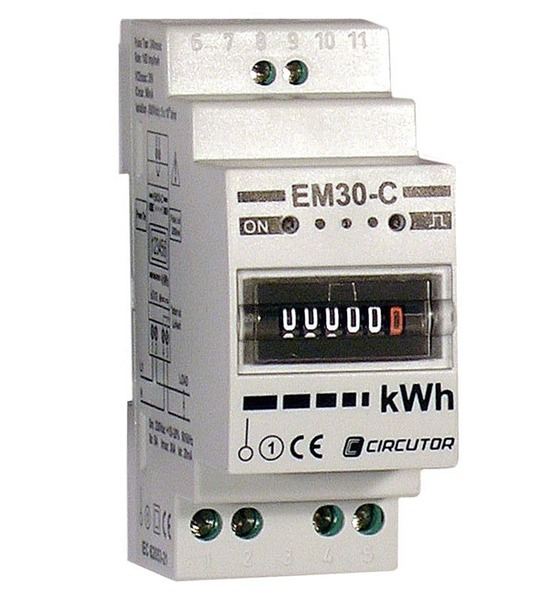
\includegraphics[width=0.25\columnwidth]{img/contatore.jpg}
    \end{figure}
\end{frame}


\begin{frame}
\frametitle{Esercizio}
\begin{columns}
\begin{column}{.35\textwidth}
  \begin{figure}
    
\includegraphics[width=\columnwidth]{img/phon.jpg}
  \end{figure}
\end{column}
\begin{column}{.6\textwidth}
  \begin{exampleblock}{Costo dell'utenza domestica}
    \small{
    Prova a stimare quanto costa asciugarsi i capelli utilizzando un phon da $ 2000 \, W $.}
  \end{exampleblock}
\end{column}
\end{columns}
\end{frame}


\section{$ \fem $}


\begin{frame}
  \frametitle{La forza elettromotrice nei generatori ideali}
  Un generatore è in grado di mantenere la sua ddp grazie alle forze interne che spostano le cariche positive verso il polo ad alto potenziale ($+$) e le negative verso il polo a basso potenziale ($-$).
  \pause
  Per ottenere questo risultato è necessario un \alert{lavoro} $ L $.\pause
  \begin{center}
\colorbox{blue!30}{$ \fem = \dfrac{L}{q} $}
\end{center}\pause
La forza elettromotrice:
\begin{itemize}
  \item si misura in volt e non è una forza ma una tensione;\pause
  \item in un generatore ideale (cioè che mantiene costante la sua ddp indipendentemente dalla corrente che lo attraversa) è la differenza di potenziale che esso mantiene tra i suoi due poli.
\end{itemize}
\end{frame}





\begin{frame}
  \frametitle{La forza elettromotrice nei generatori reali}
  Quando circola corrente in un generatore reale, una parte dell'energia del generatore serve a vincere la resistenza del moto delle cariche al suo interno (\alert{resistenza interna del generatore}).\pause\\~\\
  La differenza di potenziale effettiva sarà pertanto minore di quella ``dichiarata'', cioè la $ \fem $.
  \pause\\~\\
  Per un generatore reale, la $ \fem $ rappresenta solo la \emph{massima} differenza di potenziale che si può avere tra un polo e l'altro, cioè quella che si ha quando non passa corrente (circuito aperto).
\end{frame}





\begin{frame}
  \frametitle{Schema di un generatore reale}
  Un generatore reale presenta quindi una \emph{resistenza in serie} da considerare quando si risolve un circuito.
  \begin{columns}
\begin{column}{0.5\textwidth}  
\begin{figure}\centering
\ctikzset{bipoles/length=0.8cm}
\begin{circuitikz}[scale=0.6]
\draw (0,0) to[battery1](1.5,0) to [R, a=$r$] (3,0) to[short, a=$-$] (5.5,0) to[short, f_<=$i$] (5.5,5) to[R, a=$R$] (-2,5) to[short, f_<=$i$] (-2,0) to[short, a=$+$] (0,0);
\draw (0,-1) to[short] (0,1) to[short] (3.5,1) to[short] (3.5,-1) to[short] (0,-1);
\draw (0,.4)to[short] (-.2,.4) to[short] (-.2,-.4) to[short] (0,-.4);
\end{circuitikz}
\end{figure}
\end{column}
\begin{column}{0.5\textwidth}
{\pause} Legge delle maglie:
\[ \fem - ri - Ri = 0 \]\pause
da cui:
\[ i = \frac{\fem}{R+r} \]\pause
Prima legge di Ohm:
\[ \Delta V = \frac{R}{R+r} \fem \]
\end{column}
\end{columns}
\end{frame}








\begin{frame}
  \frametitle{$ \fem $ e differenza di potenziale}
  \[ \Delta V = \frac{R}{R+r} \fem \]
La differenza di potenziale $ \Delta V $ prodotta da un generatore sarà uguale alla sua $ \fem $ in due casi:\pause
\begin{itemize}
  \item quando $ r=0 $, cioè per i generatori ideali;\pause
  \item quando la resistenza del circuito è infinitamente grande, cioè in un circuito aperto in cui non passa corrente:
  \[ \lim_{R \rightarrow + \infty} \frac{R}{R+r} = \left[ \frac{\infty}{\infty} \right] = 1 \]
\end{itemize}
\end{frame}


\section{Resistività}


\begin{frame}
\frametitle{Seconda legge di Ohm}
\begin{block}{Seconda legge di Ohm}
  La resistenza di un filo conduttore è direttamente proporzionale alla sua lunghezza $ L $ e inversamente proporzionale alla sua sezione $ A $.
  \begin{center}
    \colorbox{blue!30}{$ R = \rho \cdot \dfrac{L}{A} $}
  \end{center}
  Il coefficiente $ \rho $ è detto \alert{resistività} e dipende dal materiale di cui è fatto il filo e dalla sua temperatura. Si misura in $ \Omega \cdot m $.
\end{block}
\begin{figure}
  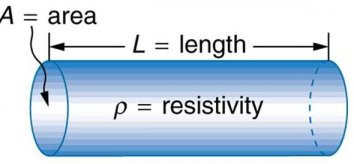
\includegraphics[width=.4\columnwidth]{img/ohm2.jpg}
\end{figure}
\end{frame}



\begin{frame}
\frametitle{Resistività a $ 293 \, K $}
\begin{table}[htb]\centering\footnotesize
  \begin{tabular}{rc}\toprule
  \textbf{Materiale} & \textbf{Resistività a $ 20\, ^\circ C$ [$ \Omega \cdot m $]}\\\midrule
  alluminio & $ 2,8 \times 10^{-8} $\\\addlinespace[1em] 
  ferro     & $ 1,0 \times 10^{-7} $\\\addlinespace[1em]
  rame      & $ 1,7 \times 10^{-8} $\\\addlinespace[1em]
  silicio   & $ 1,0 \times 10^{2}-1,0 \times 10^{3} $\\\addlinespace[1em]
  vetro     & $ 10^{10}-10^{14} $\\\bottomrule
  \end{tabular}
  \end{table}\pause

  ~

Conoscere il valore della resistività permette di dire se un certo materiale è un buon conduttore (come il rame) e un buon isolante (come il vetro).\pause

~

Le sostanze intermedie (come il silicio) sono dette \alert{semiconduttori}.
\end{frame}




%SUPERCONDUTTORI E SEMICONDUTTORI


\section{RC}


\begin{frame}
\frametitle{Circuito RC}
Un circuito RC è in circuito in cui abbiamo in serie un generatore di tensione, una resistenza e un condensatore, oltre ad un interruttore.

\begin{figure}\centering
\ctikzset{bipoles/length=1.2cm}
\begin{circuitikz}[scale=0.7]
\draw (0,0) to[switch] (0,4);
\draw (0,0) to[battery1, a=$\Delta V$] (6,0);
\draw (0,4) to[R, l=R] (6,4);
\draw (6,4) to[C, l=$C$] (6,0);
\end{circuitikz}
\end{figure}\pause
Quando chiudiamo l'interruttore la corrente inizia a scorrere nel circuito, caricando il condensatore. La corrente diminuisce man mano che il condensatore si carica.
\end{frame}

\begin{frame}
\frametitle{Carica del condensatore}
Sia la corrente sia la carica sul condensatore \alert<1>{dipendono dal tempo} e sono delle funzioni esponenziali:

\begin{columns}
\begin{column}{.4\textwidth}
  \begin{center}
    \colorbox{blue!30}{$ q(t) = C \Delta V \cdot (1-e^{-\frac{t}{RC}}) $}
  \end{center}
\end{column}
\begin{column}{.4\textwidth}
  \begin{center}
    \vspace*{1.2em}
    \colorbox{blue!30}{$ i(t) = \frac{\Delta V}{R} \cdot e^{-\frac{t}{RC}} $}
  \end{center}
\end{column}
\end{columns}
\begin{columns}
\begin{column}{.4\textwidth}
  \begin{figure}
    \begin{tikzpicture}[xscale=.3,yscale=1.2]
      \node [left] at (0,2) {{\scriptsize $ q(t) \, [C] $}};
      \node [below] at (10,0) {{\scriptsize $ t \, [s] $}};
      \draw [->] (-1,0) -- (10,0);
      \draw[smooth, dashed, domain=0:8.5] plot (\x,{1.5});
      \draw [->] (0,-.1) -- (0,2);
      \draw[smooth, blue, thick, domain=0:8.5] plot (\x,{1.5 - 1.5*e^(-.5*\x)});
      \draw (7.5,-.1) -- (7.5,.1);
      \draw [dotted] (7.5,0) -- (7.5,1.5);
      \node [below] at (7.5,0) {{\scriptsize $ 5RC $}};
      \end{tikzpicture}
  \end{figure}
\end{column}
\begin{column}{.4\textwidth}
  \begin{figure}
  \begin{tikzpicture}[xscale=.3,yscale=1.2]
      \node [left] at (0,2) {{\scriptsize $ i(t) \, [A] $}};
      \node [below] at (10,0) {{\scriptsize $ t \, [s] $}};
      \draw [->] (-1,0) -- (10,0);
      \draw [->] (0,-.1) -- (0,2);
      \draw[smooth, red, thick, domain=0:8.5] plot (\x,{1.5*e^(-.5*\x)});
      \draw (7.5,-.1) -- (7.5,.1);
      \node [below] at (7.5,0) {{\scriptsize $ 5RC $}};
      \end{tikzpicture}
  \end{figure}
\end{column}
\end{columns}\pause

~

Si considera il condensatore praticamente carico dopo un tempo $ t = 5 RC $ (con $ RC $ detto ``tempo caratteristico'').
\end{frame}


\begin{frame}
\frametitle{Scarica del condensatore}
Se apriamo il circuito, il condensatore \alert<1>{si scarica}.

\begin{columns}
\begin{column}{.4\textwidth}
  \begin{figure}
    \colorbox{blue!30}{$ q(t) = C \Delta V \cdot e^{-\frac{t}{RC}} $}

    ~

    \begin{tikzpicture}[xscale=.3,yscale=1.2]
      \node [left] at (0,2) {{\scriptsize $ q(t) \, [C] $}};
      \node [below] at (10,0) {{\scriptsize $ t \, [s] $}};
      \draw [->] (-1,0) -- (10,0);
      \draw [->] (0,-.1) -- (0,2);
      \draw[smooth, blue, thick, domain=0:8.5] plot (\x,{1.5*e^(-.5*\x)});
      \draw (7.5,-.1) -- (7.5,.1);
      \node [below] at (7.5,0) {{\scriptsize $ 5RC $}};
      \end{tikzpicture}
  \end{figure}
\end{column}
\begin{column}{.4\textwidth}
  \begin{figure}
    \colorbox{blue!30}{$ i(t) = - \frac{\Delta V}{R} \cdot e^{-\frac{t}{RC}} $}

    ~

    \begin{tikzpicture}[xscale=.3,yscale=1.2]
      \node [left] at (0,2) {{\scriptsize $ i(t) \, [A] $}};
      \node [below] at (10,0) {{\scriptsize $ t \, [s] $}};
      \draw [->] (-1,0) -- (10,0);
      \draw [<-] (0,-.1) -- (0,2);
      \draw[smooth, red, thick, domain=0:8.5] plot (\x,{1.5*e^(-.5*\x)});
      \draw (7.5,-.1) -- (7.5,.1);
      \node [below] at (7.5,0) {{\scriptsize $ 5RC $}};
      \end{tikzpicture}
  \end{figure}
\end{column}
\end{columns}\pause

~

Si considera il condensatore praticamente scarico dopo un tempo $ t = 5 RC $.
\end{frame}



\begin{frame}
\frametitle{Esercizio}
\begin{exampleblock}{Circuito RC}
  \small{
    In un circuito, alimentato da una batteria che fornisce una differenza di potenziale di $ 4,5 \, V $, sono collegati in serie un condensatore di capacità $ C $ e un resistore di resistenza $ R = 70 \, \Omega $. Il tempo caratteristico del circuito è di $ 1,3 \, s $. Calcola:
    \begin{itemize}
      \item la capacità del condensatore;\hspace*{\fill}[$ 1,9 \times 10^{-5} \, F $]
      \item l'intensità della corrente nel circuito dopo un intervallo di tempo di $ 2,6 \, s $\hspace*{\fill}[$ 8,7 \times 10^{-3} \, A $]
    \end{itemize}}
\end{exampleblock}
\end{frame}


\end{document}
